\documentclass[a4paper]{article}

\usepackage[french]{babel}
\usepackage[T1]{fontenc}
\usepackage[utf8]{inputenc}
\usepackage{amsmath}
\usepackage{graphicx}
\usepackage{lmodern}
\usepackage[left=3cm, right=3cm, bottom=4cm, top=4cm]{geometry}
\usepackage{array}
\usepackage{pdfpages}
\usepackage{listings}
\usepackage{algorithm}
\usepackage{algorithmic}
\usepackage{sidecap}
\usepackage{pdflscape}
\usepackage{hyperref}
\usepackage{tipa}
\usepackage{multirow}
\usepackage[gen]{eurosym}
\usepackage{float}
\usepackage{color}
\definecolor{bo_vert}{rgb}{0,0.65,0}
\definecolor{nouvo_rouge}{rgb}{0.65,0,0}
\usepackage{pifont}
\DeclareUnicodeCharacter{20AC}{\euro{}}

\usepackage{hyperref}
\hypersetup{    
    colorlinks,
    citecolor=black,
    filecolor=black,
    linkcolor=black,
    urlcolor=black
}

\title{Rapport final}

\author
{
    Pierre-Marie {\sc Airiau}\\
    Valentin {\sc Esmieu}\\
    Maud {\sc Leray}\\
    %Hoel {\sc Kervadec}\\
    %Florent {\sc Mallard}\\
    %Corentin {\sc Nicole}\\
    %ON VOUS AIME LES COPAINS
}

\date{\today}

\newcommand{\pagevierge}[0]{\newpage\thispagestyle{empty}\null\newpage}
\newcommand{\glasir}[0]{Glasir}
\newcommand{\ttable}[0]{{\sc Table}}
\newcommand{\ffigure}[0]{{\sc Figure}}

\newcommand{\nomRepart}[1]{\multicolumn{2}{c||}{\textbf{#1}}}
\newcommand{\nomRepartt}[1]{\multicolumn{2}{c|}{\textbf{#1}}}

\begin{document}
    % Ouh c'est sale.
    \hypersetup{pageanchor=false}
    
\includepdf[pages=1]{figure/couv.pdf}
    \hypersetup{pageanchor=true}
    
    \newpage
    \thispagestyle{empty}
    \mbox{}
    
    \newpage
    
    \setcounter{tocdepth}{2}
    \tableofcontents
    \setlength{\parskip}{10pt}
    
    \newpage
    \thispagestyle{empty}
    \mbox{}

	\newpage
    \section{Remerciements}

Ce projet terminé, nous souhaitons adresser nos remerciements à certaines personnes qui nous ont aidés et soutenus :   

Nous remercions en premier lieu nos camarades Corentin {\sc Nicole}, Hoel {\sc Kervadec} et Florent {\sc Mallard}, qui ont partagé avec nous la phase de conception de ce projet, et qui ont contribué à sa mise en place et sans nul doute à son aboutissement.

Nous souhaitons ensuite remercier particulièrement nos encadrants, Mme Barbara {\sc Kordy} et M. Gildas {\sc Avoine}, qui se sont toujours montrés disponibles, impliqués et d'une aide précieuse. Un grand merci à eux pour leurs conseils avisés.

Nous remercions aussi vivement M. Piotr {\sc Kordy}, l'un des concepteurs d'ADTool, qui a su se montrer disponible pour répondre à nos interrogations concernant le logiciel.

Nous tenons aussi à remercier les élèves de 5ème année du département Informatique, qui nous ont fourni un ensemble d'ADTrees assez conséquents réalisés lors d'un TP. Grâce à eux, nous avons pu tester notre logiciel sur des ADTrees assez représentatifs d'une situation d'analyse de sécurité réelle.

Enfin, nous adressons nos remerciements à M. Jean-Louis {\sc Pazat}, pour le temps qu'il a consacré à la lecture de nos rapports et au suivi de notre projet.

    \newpage
    \chapter{Contexte}

	\section{Un contexte mondial}

	Le bon fonctionnement des transports en commun dépend de nombreux facteurs. Qu'il soit humain, ou bien technique, le moindre dysfonctionnement impactera le système entier très rapidement. Ainsi, un simple tour d'horizon de la presse internationale fait vite remonter à la surface de nombreux cas de paralysie des transports publics urbains dans le monde entier.

		\subsection{ Les risques d'atteinte aux passagers }

	Parmi tous les cas de paralysie, les plus marquants à l'échelle internationale sont ceux impliquant des dégâts humains importants parmi les passagers. Il s'agit, dans la plupart des cas, d'attaques terroristes. Bien qu'ils soient relativement rares, le lourd bilan humain de ces attentats marque durablement les esprits.

	C'est le cas de l'attentat à la bombe dans la gare Saint-Michel du train inter-urbain parisien, le 25 juillet 1995, qui provoqua la mort de 8 personnes\cite{stmichel}. L'attaque la plus marquante de l'histoire fut celle du 7 juillet 2005 dans la ville de Londres. Quatre attentats-suicides dans différentes rames de métro provoquent la mort de 56 personnes et en blessent 700 autres. \cite{london_attacks}.

    	\subsection{ Le risque des mouvements sociaux }
    	
	Si ces attaques sont impressionantes et marquantes pour la population, elles restent minoritaires dans les cas de paralysie. Un rapide tour d'horizon de la presse internationale nous montre que la majorité des cas de blocage des transports en communs sont provoqués par le personnel des compagnies gérant ces transports. En effet, lors de conflits sociaux, le personnel possède un énorme moyen de pression sur la hiérarchie car il peut bloquer l'intégralité du traffic en se mettant en grève. 

	C'est le cas à Londres, où un plan de fermeture des guichets du métro a provoqué une grève massive le 28 avril 2014. Cela a entraîné la fermeture des deux tiers des stations et la diminution du traffic de 50\% \cite{tubeApril}. Mais aussi à San Fransisco, en juillet et octobre 2013, où une grève du réseau ferré interurbain (forte de ses 400 000 milles passagers par jour) a paralysé la ville pendant plusieurs jours. \cite{SFbart}

	\section{La situation en France}
	
	En France, il arrive aussi que les réseaux de transports en commun soient mis en difficulté. Les archives ne contiennent pas de traces de graves attentats tels que cités précédemment : la plupart du temps, les troubles sont dûs à des grèves du personnel pouvant refléter différentes réclamations.
	
	\subsection{ Les évènements notables dans tout le pays }

	Commençons par Marseille en décembre 2013, où les conducteurs ont réussi à bloquer la quasi-totalité du réseau pendant plus de deux jours. Ils protestaient contre les salaires, la pénibilité en fin de carrière et la suppression de deux jours de congés. Cela est également arrivé à Lille en mai 2014, où le tramway et les bus ont été immobilisés par les traminots demandant une hausse des salaires.

	Mais parfois, les grèves sont la conséquence de certains incidents survenus lors des trajets. Le plus souvent, il s'agit d'agressions sur le personnel, qui sont plus fréquentes qu'on ne pourrait le penser.

	À Dunkerque en mai 2013 par exemple, un chauffeur subit une agression de la part de voyageurs, qui l'ont poursuivi en voiture jusqu'au terminus de la ligne. Arrivés là, équipés d'extincteurs, ils ont bloqué le bus et menacé ses occupants. La CGT a été avertie, une plainte a été déposée et les conducteurs ont exercé leur droit de retrait, paralysant ainsi le réseau pendant toute une journée.

	C'est ensuite à Douai, en septembre de la même année, que trois contrôleurs sont agressés lors d'un contrôle par une vingtaine de personnes. Des coups sont échangés, les trois hommes finissent à l'hôpital avec des contusions et une entorse au poignet pour l'un d'entre eux. L'ensemble des contrôleurs du réseau exerce alors son droit de retrait, bloquant celui-ci pendant une journée entière.

	Mais qu'en est-il au sein de l'agglomération rennaise, qui nous intéresse tout particulièrement dans le cadre de ce projet ? Commençons par décrire le réseau de transports actuellement en place, ainsi que sa gestion.
		
		\subsection{ Le cas rennais }

	Le réseau de transports rennais est constitué d'une ligne de métro (une deuxième étant en construction) et d'un réseau de bus. Ces deux éléments sont gérés par le STAR (Service des Transports en commun de l'Agglomération Rennaise), qui dépend de la société Keolis Rennes. Le STAR a également mis en place depuis quelques années un système de vélos en libre-service : les vélos STAR. Les usagers peuvent accéder aux différents services du STAR par plusieurs moyens : en achetant des tickets à l'unité (pour bus et métro), ou en utilisant une carte d'abonné rechargeable (la carte Korrigo). 
	
	L'information aux voyageurs passe par 870 écrans dans les bus, 70 dans les stations de métro et 50 bornes d’informations voyageurs (BIV) dans les abribus. Le système d’aide à l’exploitation et à l’information des voyageurs (SAEIV) permet d’indiquer en temps réel le passage du prochain bus, les perturbations, les correspondances, la disponibilité des Vélos STAR… Ces données sont disponibles en open data, et consultables via un service mobile mis à disposition par le STAR.

	Toute cette organisation n'est cependant pas à l'abri des incidents et présente quelques failles : voici un récapitulatif des paralysies les plus importantes que nous avons trouvées.

	En juillet 2009, la ligne de métro a été bloquée pendant près de 20h à la suite d'un violent orage provoquant l'inondation des voies de circulation. Ceci n'est certes pas une attaque volontaire mais cela reste une faiblesse du système qu'il nous a paru intéressant de relever. 

	C'est ensuite en avril 2012 que le réseau STAR entier a été paralysé, en pleine heure de pointe, suite à l'agression d'un chauffeur. À l'époque, la direction recensait 18 agressions depuis le début de l'année, et promettait un redéploiement de ses agents de médiation et de prévention. Une mesure insuffisante pour la CFDT, qui réclamait "une police dédiée aux transports".

	Environ un mois plus tard, en mai, la ligne de métro a été bloquée dès 5h30 du matin. Selon le STAR, il s’agirait d’un problème informatique entre le centre de commandement du métro et les rames : la liaison qui permet de contrôler les rames à distance ne fonctionnait plus. Un service de bus a été mis en place pour limiter les conséquences.

	Ces quelques faits montrent bien l'importance pour le STAR de la mise en place d'un outil d'évaluation des risques, qui comporterait également un répertoire de défenses à utiliser pour contrer ces derniers.


    \newpage
    \section{Rectificatifs du rapport de spécifications fonctionnelles}
\label{sec:rect}

Cette section a pour but d'énoncer et de justifier les différences constatées entre les fonctionnalités prévues dans le rapport de spécifications fonctionnelles~\cite{spec_fonc} et leur implémentation lors de la phase de développement. La {\sc sous-section}~\ref{subsec:archi} commence d'abord par énoncer les modifications les plus générales concernant l'architecture du logiciel, avant d'entrer plus en profondeur dans le code dans les sous-sections suivantes.

\subsection{Architecture générale}
\label{subsec:archi}

La {\sc Figure} \ref{fig:archiPrevue} illustre l'architecture générale imaginée lors du rapport de spécifications fonctionnelles~\cite{spec_fonc}. Suite à des contraintes techniques, notamment dûes au fait qu'un programme Java (ADTool dans notre cas) est difficilement contrôlable depuis un programme C\#, l'architecture a été revue pour correspondre à celle présentée à la {\sc Figure}~\ref{fig:archiReelle}. C'est pourquoi ADTool ne fait finalement pas partie intégrante de Glasir, mais est lancé en tant que simple \og viewer \fg{} d'ADTrees. En effet, il est impossible, depuis Glasir, de détecter des modifications faites dans ADTool, comme par exemple la modification d'une valuation de l'une des feuilles de l'ADTree. Par conséquent, la décision fut prise de désactiver toutes les fonctions d'édition dans ADTool lorsque Glasir se lance, donnant ainsi à ADTool un mode spécial baptisé \og viewmode \fg{}. Dans ce mode, l'utilisateur ne peut que visualiser un ADTree, sans pouvoir le modifier (les menus et les raccourcis clavier ont été supprimés). De plus, la bibliothèque de modèles n'est plus incluse dans Glasir : cette décision est justifiée dans la {\sc sous-section}~\ref{ssec:bib}.

		\begin{figure}[H]
            \centering
                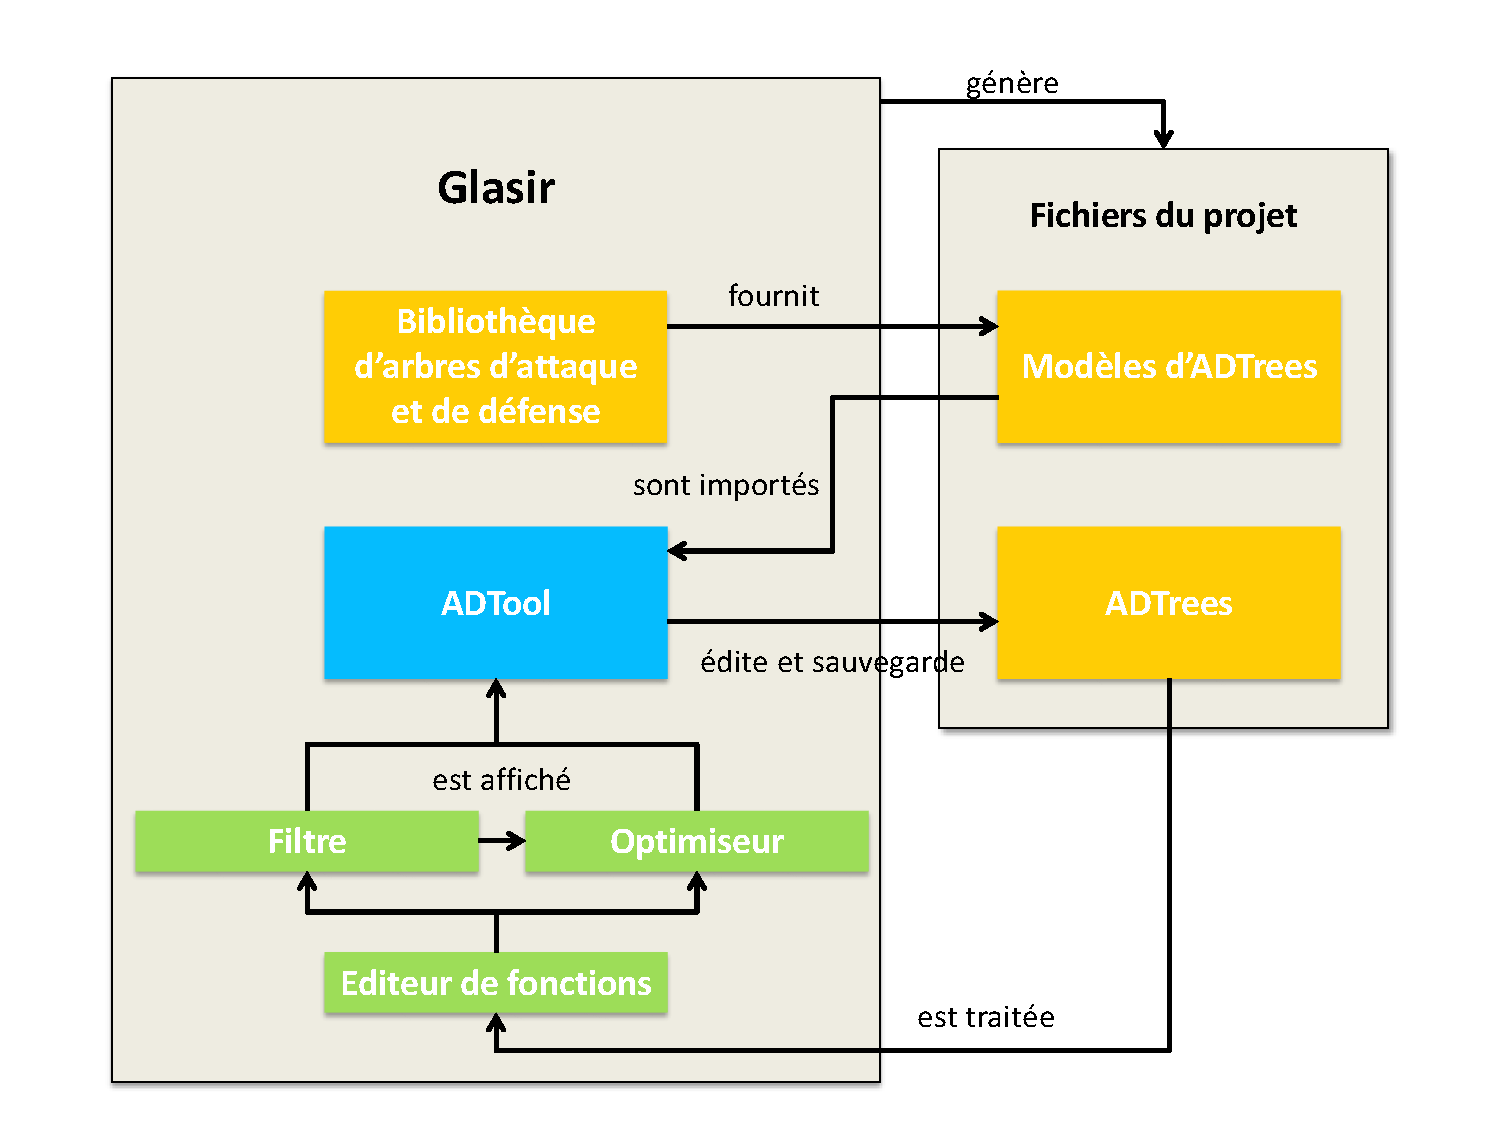
\includegraphics[width=0.8\textwidth]{figure/archiGlasir.pdf}
            \caption{Architecture initialement prévue.}
            \label{fig:archiPrevue}
        \end{figure}
	
        
        \begin{figure}[H]
            \centering
                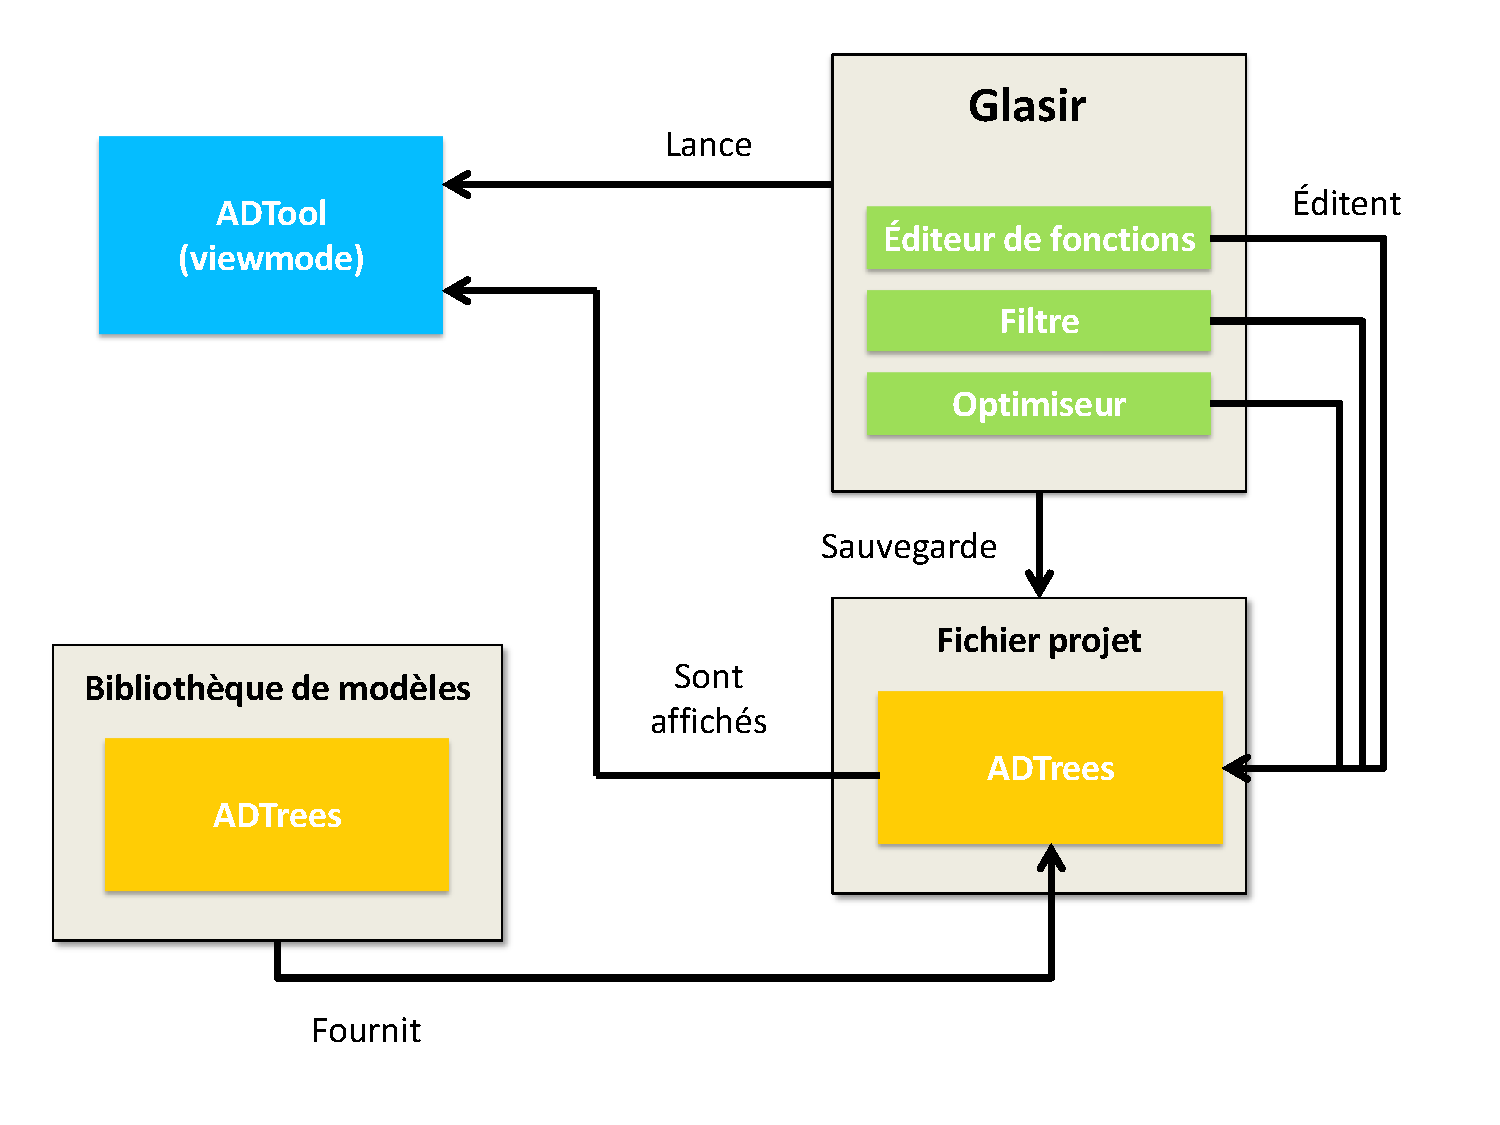
\includegraphics[width=0.8\textwidth]{figure/archiReelle.pdf}
            \caption{Architecture réelle.}
            \label{fig:archiReelle}
        \end{figure}
        
Les modules principaux de Glasir que sont l'Éditeur de fonctions, le Filtre et l'Optimiseur ont eux aussi été un peu revus par rapport à l'implémentation prévue dans le rapport de conception~\cite{conception}. Ces changements sont principalement liés à des questions de cohérence soulevées après le début du développement. Les {\sc sous-sections}~\ref{ssec:editeurFct},~\ref{ssec:implemFiltre} et~\ref{ssec:algoOptim} détaillent les modifications apportées à ces modules.

\subsection{Algorithme de l'Éditeur de fonctions}
\label{ssec:editeurFct}

\BK{Regardez la ligne 28 de mon main.tex, pour voir comment 
redéfinir le nom d'Algorithm (en anglais)  en Algorithme (en français)}

Bien que nous n'ayons pas jugé nécessaire de détailler l'algorithme de l'Éditeur de fonctions lors de la rédaction du rapport de spécifications fonctionnelles~\cite{spec_fonc}, celui-ci s'est révélé plus délicat à implémenter que prévu. Son nouveau fonctionnement est donc détaillé ci-après, par une présentation de l'{\sc algorithme}~\ref{algo:functionEdition} qui a été effectivement implémenté.

\BK{Si vous voulez changer IN en \textbf{in} dans les algorithmes, 
je vous montre comment faire dans la deuxième ligne d'algorithme ci-dessous, il suffit de mettre 
'\textbf{in}' au lieu de 'IN' (voir le fichier 
rectificatifs.tex)}

	\begin{algorithm}[H]
            \caption{functionEdition(racine, param1, param2, function)}
            \label{algo:functionEdition}
            \begin{algorithmic}
		\IF{type(racine) == defense}
			\FORALL{sub \textbf{in} fils(racine)}
				\STATE functionEdition(sub, param1, param2, function)
			\ENDFOR
			\RETURN
		\ENDIF
		\STATE
		\IF{type(racine) == feuille}
			\STATE p1 = param1(racine)
			\STATE p2 = param2(racine)
			\STATE newParam(racine) = function(p1,p2)
			\RETURN
		\ELSE
			\FORALL{sub IN fils(racine)}
				\IF {(type(sub) == defense}
					\STATE p1 = param1(racine)
					\STATE p2 = param2(racine)
					\STATE newParam(racine) = function(p1,p2)
				\ENDIF
				\STATE functionEdition(sub, param1, param2, function)
			\ENDFOR
		\ENDIF
            \end{algorithmic}
        \end{algorithm}

 Les notations non explicites de l'{\sc algorithme}~\ref{algo:functionEdition} sont présentées ci-dessous :
        \begin{itemize}
            \item \verb|racine| correspond au nœud racine de l'arbre ou sous-arbre manipulé ;
            \item \verb|param1| est une fonction renvoyant la valeur du 1\ier{} paramètre qui nous intéresse pour un nœud donné ;
            \item \verb|param2| est une fonction renvoyant la valeur du 2\ieme{} paramètre qui nous intéresse pour un nœud donné ;
            \item \verb|function| est une fonction calculant un résultat à partir de deux paramètres ;
            \item \verb|fils| est une fonction renvoyant la liste des fils du nœud passé en paramètre ;
            \item \verb|mode| précise si il s'agit d'un nœud disjonctif ou conjonctif ;
            \item \verb|type| précise si il s'agit d'un nœud d'attaque ou de défense, ou bien d'une feuille.
        \end{itemize}

    L'algorithme de l'éditeur de fonctions est donc un algorithme récursif, qui cherche les feuilles de l'ADTree pour ajouter le nouveau paramètre à celle-ci. \BK{à celles-ci (au pluriel, s'il s'agit des feuilles)}

\subsection{Algorithme du Filtre}
\label{ssec:implemFiltre}

L'algorithme original du Filtre \BK{, représenté par l'{\sc algorithme}~\ref{algo:filtre},} comportait quelques erreurs, telles que la possibilité de conserver des sous-n\oe{}uds d'un n\oe{}ud conjonctif qui ne respectaient pas la condition de filtrage. Cet algorithme, 
\BK{Je supprimerai la référence à l'algo original ici et la mettrai dans la première phrase de ce paragraph}
l'{\sc algorithme}~\ref{algo:filtre}, a donc été corrigé en conséquence pour devenir l'{\sc algorithme}~\ref{algo:filtreReel} qui a été implémenté.

 	\begin{algorithm}[H]
            \caption{filtre(racine, rules)}
            \label{algo:filtre}
            \begin{algorithmic}
                \FOR{r in rules}
                    \IF{not r(racine)}
                        \STATE delete(r) // will delete subtrees as well
                        \RETURN
                    \ENDIF
                \ENDFOR
                \STATE
                \FOR{n in fils(racine)}
                    \STATE filtre(n, rules)
                \ENDFOR
            \end{algorithmic}
        \end{algorithm}
        

 	\begin{algorithm}[H]
            \caption{filtre(racine, param, valLim)}
            \label{algo:filtreReel}
            \begin{algorithmic}
	\STATE val = param(racine)
	\STATE
	\IF {pire(val, valLim)}
		\STATE delete(racine) // will delete subtrees as well
		\RETURN
	\STATE
	\ELSE
		\IF{mode(racine) == et}
			\FORALL{sub IN fils(racine)}
				\STATE subval = sub.param
				\STATE filtre(sub, param, valLim+subval-val)
			\ENDFOR
		\ELSE
			\FORALL{sub IN fils(racine)}
				\STATE filtre(sub, param, valLim)
			\ENDFOR
		\ENDIF
	\ENDIF
            \end{algorithmic}
        \end{algorithm}

    Dans l'{\sc algorithme}~\ref{algo:filtreReel}, \verb|valLim| est la valeur limite (maximale ou minimale selon les cas) acceptée pour le paramètre \verb|param| que l'on désire dans l'arbre filtré peu importe le chemin envisagé, et  \verb|pire| est une fonction renvoyant vrai \BK{\emph{vrai}} si son premier paramètre est moins bon que son second pour le domaine de valuation considéré, et 
		faux \BK{\emph{faux}} sinon.
\BK{Je ne suis pas sûre que le paragraphe ci-dessus est compréhensible}

\subsection{Algorithme de l'Optimiseur}
\label{ssec:algoOptim}

    L'algorithme initial de l'Optimiseur, tel que décrit dans le rapport de spécifications fonctionnelles~\cite{spec_fonc}, est rappelé par l'{\sc algorithme}~\ref{algo:opti}.

         \begin{algorithm}[H]
            \caption{opti(racine, param)}
            \label{algo:opti}
            \begin{algorithmic}
                \STATE l\_fils = fils(racine)
                \IF{vide(l\_fils)}
                    \RETURN
                \ENDIF
                \STATE
                \IF{mode(racine) == ou}
                    \STATE v = param(racine)

                    \FOR{n in l\_fils}
                        \IF{not defense(n) and param(n) != v}
                            \STATE delete(n) // will delete subtrees as well
                        \ENDIF
                    \ENDFOR
                \ENDIF
                \STATE
                \FOR{n in fils(racine)}
                    \STATE opti(n, param)
                \ENDFOR
            \end{algorithmic}
        \end{algorithm}

Après réflexion, 
\BK{Je n'aime pas de formulation 'après réflexion'. Cela fait entendre que vous n'avez pas assez réfléchi auparavant. Essayez de réécrire ça autrement, par exemple:\\
Après avoir implémenté le Filtre, il est apparu que l'Optimiseur pouvait être implémenté de manière bien plus simple. L'{\sc algorithme}~\ref{algo:optiReel}
représente la solution qui a finalement été  choisi pour coder l'Optimiseur. }
il est apparu que l'{\sc algorithme}~\ref{algo:opti} pouvait être implémenté de manière bien plus simple, en se servant du Filtre. Ce nouvel algorithme n'impactant pas le résultat obtenu, c'est donc lui qui a finalement été choisi et codé selon l'{\sc algorithme}~\ref{algo:optiReel}.

	\begin{algorithm}[H]
            \caption{opti(racine, param)}
            \label{algo:optiReel}
            \begin{algorithmic}
		\STATE v = param(racine)
		\STATE filtre(racine, param, v)
            \end{algorithmic}
        \end{algorithm}

    La présente section a permis de décrire les différences constatées à la fin du projet entre les promesses du rapport de spécifications fonctionnelles~\cite{spec_fonc} et l'implémentation réelle. Un autre rapport avait été rédigé avant le début du développement, celui de conception~\cite{conception}. Là encore, des écarts sont constatés avec ce qui a été codé, c'est ce dont fait état la {\sc section}~\ref{sec:rectConc}. 

\newpage
\section{Rectificatifs du rapport de conception}
\label{sec:rectConc}
    
    Cette section a pour objectif de comparer les fonctionnalités décrites lors du rapport de conception~\cite{conception} à celles qui ont été ensuite implémentées.

	\subsection{Affichage multiple des paramètres}

    Cette nouveauté n'a finalement pas été mise en place. En effet, l'étude approfondie du code source d'ADTool a montré qu'un tel changement aurait nécessité une refonte quasi-totale de la structure du logiciel. De telles modifications auraient demandé un temps de travail bien trop conséquent comparé au temps disponible pour la réalisation du projet. De toute manière, l'intérêt de ce nouvel affichage avait finalement été remis en cause : le risque de perdre en clarté et en lisibilité lors de la manipulation des ADTrees avait semblé trop important.

	\subsection{Couper/copier/coller}

	La {\sc Figure} \ref{fig:copypastePrevu} rappelle le \BK{la fonctionnalité de} couper/copier/coller \BK{telle qu'}imaginé lors du rapport de conception~\cite{conception}. Après avoir mieux pris connaissance de la structure interne d'ADTool, il a paru beaucoup plus simple de réaliser cette fonctionnalité comme illustré sur la {\sc Figure} \ref{fig:copypasteReel}.
	
	
		\begin{figure}[H]
            \centering
                
\includegraphics[width=0.8\textwidth]{figure/copiercoller.png}
            \caption{Diagramme de classes prévu pour le couper/copier/coller.}
            \label{fig:copypastePrevu}
        \end{figure}
        
        \begin{figure}[H]
            \centering
                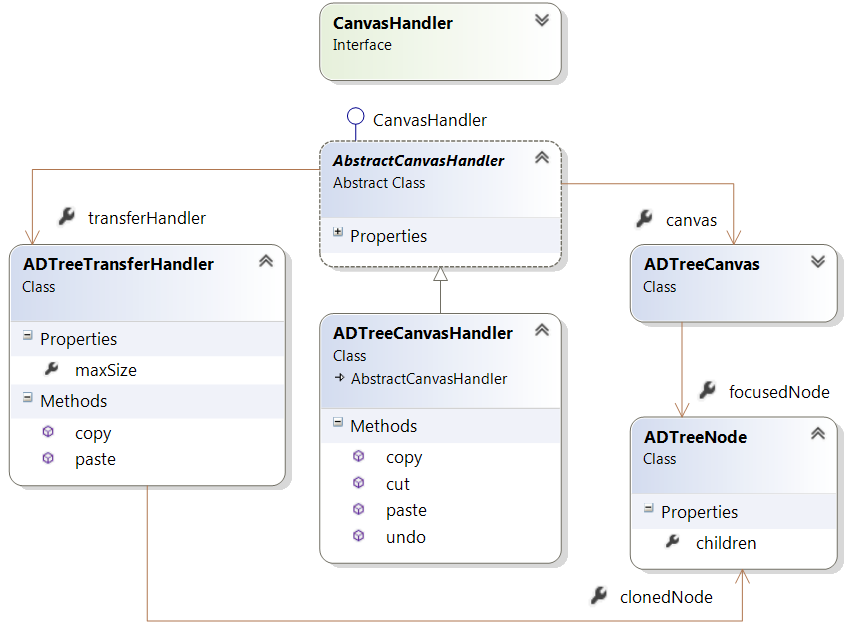
\includegraphics[width=0.9\textwidth]{figure/copiercollerReel.png}
            \caption{Diagramme de classes réellement implémenté pour le couper/copier/coller.}
            \label{fig:copypasteReel}
        \end{figure}

        Dans ADTool, un ADTree est en réalité un \emph{ADTreeNode} possédant des fils, qui sont eux-mêmes des \emph{ADTreeNode}. L'ADTree courant est affiché à l'écran via un \emph{ADTreeCanvas}. Les actions au clavier et à la souris réalisées par l'utilisateur sont captées par la classe \emph{AbstractCanvasHandler}, qui possède le \emph{ADTreeCanvas} sur lequel agit l'utilisateur. Il a donc été ajouté à l'\emph{AbstractCanvasHandler} un attribut de \emph{ADTreeTransferHandler}, une nouvelle classe qui contient les méthodes de copie et de collage d'un \emph{ADTreeNode}. Ainsi, lorsque l'utilisateur lance la commande \og couper \fg{}, par exemple, cette dernière est captée par la classe \emph{CanvasHandler} qui demande alors à sa classe parente (\emph{AbstractCanvasHandler}) de récupérer l'\emph{ADTreeNode} à couper (il s'agit de l'attribut \emph{focusedNode} de \emph{ADTreeCanvas}). L'\emph{ADTreeTransferHandler} se charge ensuite de l'opération de copie en stockant dans \emph{clonedNode} un clone de l'\emph{ADTreeNode} coupé. Dans le cas de l'action \og couper \fg{}, la suppression de l'ADTree coupé est gérée en interne par l'\emph{AbstractCanvasHandler}. Pour le collage, les opérations sont sensiblement identiques, sauf que le clone stocké par l'\emph{ADTreeTransferHandler} est restitué à l'\emph{AbstractCanvasHandler} qui se charge de l'ajouter à son \emph{ADTreeCanvas}.
       
	\subsection{Annulation des dernières actions}

		 La {\sc Figure}~\ref{fig:ctrlzPrevu} illustre l'implémentation de l'annulation de la dernière action telle qu'imaginée lors du rapport de conception~\cite{conception} (dans lequel il n'était pas prévu de pouvoir effectuer plusieurs annulations à la suite \BK{C'est une information importante, car vous avez implémenté mieux que prévu. A votre place, je supprimerais  les parenthèses}). De la même façon que pour le couper/copier/coller, la structure d'ADTool a mené \BK{'a mené' ou 'a emmené' ?} à implémenter l'annulation différemment, comme indiqué sur la {\sc Figure}~\ref{fig:ctrlzReel}. 
		 
        \begin{figure}[H]
            \centering
                
\includegraphics[width=0.8\textwidth]{figure/ctrlz.png}
            \caption{Diagramme de classes prévu pour l'annulation des dernières actions.}
            \label{fig:ctrlzPrevu}
        \end{figure}
        
        \begin{figure}[H]
            \centering
                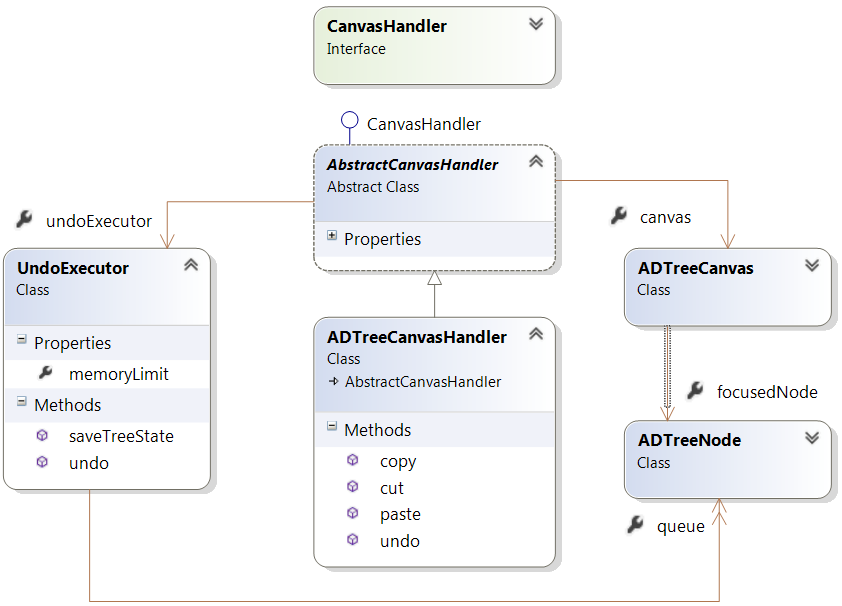
\includegraphics[width=0.8\textwidth]{figure/ctrlzReel.png}
            \caption{Diagramme de classes réel\BK{lement implémenté} pour l'annulation des dernières actions.}
            \label{fig:ctrlzReel}
        \end{figure}

        En effet, associer chaque action à une classe se révélait trop fastidieux, étant donné le grand nombre d'actions possibles. L'\emph{AbstractCanvasHandler} se voit donc doté d'un attribut de \emph{UndoExecutor}, une nouvelle classe qui contient les méthodes d'annulation. Lorsque l'utilisateur réalise une action, un clone de l'ADTree courant est stocké dans la pile de l'\emph{UndoExecutor}. Les clones sont dépilés et rechargés dans l'\emph{ADTreeCanvas} lorsque l'utilisateur utilise la fonctionnalité d'annulation. Afin d'éviter une saturation de la mémoire, la pile ne peut contenir qu'un certain nombre de clones de l'ADTree, supprimant si besoin le plus ancien pour pouvoir ajouter le plus récent. Il est à noter que plus l'ADTree est petit, plus le nombre d'actions annulables est grand, car la pile peut contenir plus de clones avant d'arriver à saturation. Dans le pire des cas, si l'ADTree est immense 
\BK{je dirais plutôt 'conséquent' ou 'grand'}				
				(dans notre cas, s'il contient plus de 1000 n\oe{}uds), seule la dernière action sera annulable. 

	\subsection{Bibliothèque de modèles}
    \label{ssec:bib}
		La {\sc Figure} \ref{fig:library} illustre l'implémentation de la bibliothèque de modèles telle qu'imaginée lors du rapport de conception~\cite{conception}. 
		
		\begin{figure}[H]
            \centering
                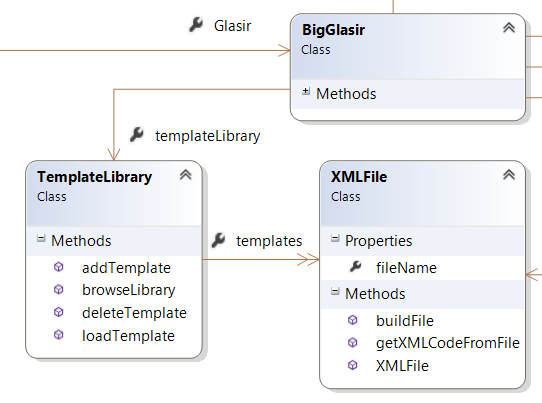
\includegraphics[width=0.8\textwidth]{figure/library.png}
            \caption{Diagramme de classes prévu pour la bibliothèque de modèles.}
            \label{fig:library}
        \end{figure}

        Finalement, cette bibliothèque se présente comme un simple dossier (fourni avec Glasir) contenant les modèles d'ADTrees. Ceux-ci portent sur le thème des transports en commun, ce qui correspond à l'étude de cas dans le cadre de ce projet mais ne doit pas restreindre l'utilisation de Glasir. C'est pourquoi il a été décidé de la fournir séparée du logiciel, pour que ce dernier reste adapté à l'analyse en sécurité de n'importe quel système.
   	
    \newpage
    \section{Compte-rendu des tests}

On s'est donné deux versions intermédiaires pour être sûr de ce qu'on faisait.
\subsection{Version 0.1}
Après version 0.1 : Problème machine vierge, problème éditeur fonctions

\subsection{Version 0.2}
Après version 0.2 : problème config jar, regarder le compte rendu 2015-chaipakoi
    
    \newpage
    \section{État de Glasir à la conclusion du projet}
\label{sec:etatFinal}

Cette section présente l'état dans lequel Glasir a été livré à l'issue du projet. On présente ici un récapitulatif des objectifs initiaux et leur état d'achèvement dans la {\sc sous-section}~\ref{subsec:objOK}, avant d'évoquer en {\sc sous-section}~\ref{subsec:encorePlusMieux} des améliorations à envisager.

\subsection{Tenue des objectifs}
\label{subsec:objOK}

Cette sous-section récapitule en premier lieu les accomplissements relatifs à Glasir, avant de mettre en évidence ceux concernant ADTool.

\subsubsection{Glasir}
\label{sssec:obj_glasir}

L'objectif du projet était de fournir à des experts en sécurité, familiers avec le formalisme des ADTrees, une solution logicielle pour analyser et exploiter ces derniers. L'utilisation de cette solution logicielle, Glasir, devait se faire au moyen d'un ensemble de \og modules \fg{} constituant les fonctionnalités d'analyse des ADTrees, au sein d'une interface graphique simple et claire. L'interface imaginée pour répondre à ces besoins est celle de la {\sc figure}~\ref{fig:InterfaceGlasir}.

    \begin{figure}[H]
        \centering
        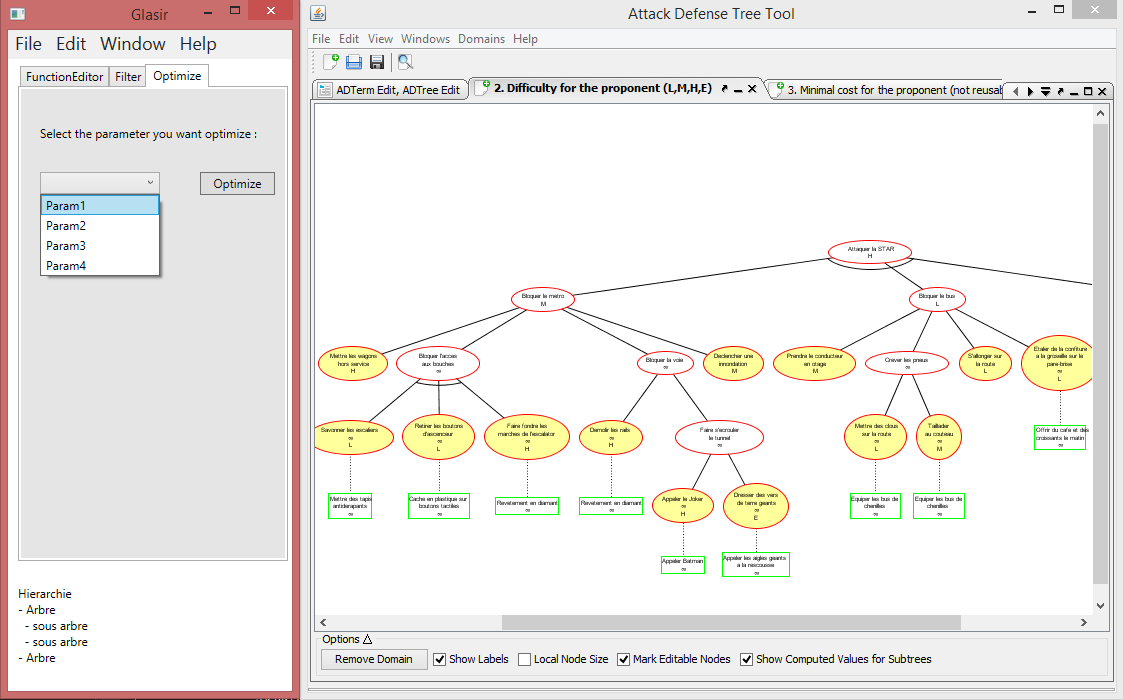
\includegraphics[height=0.75\textwidth]{figure/interface.png}
        \caption{Interface du logiciel Glasir.}
        \label{fig:InterfaceGlasir}
    \end{figure}

L'interface graphique de Glasir a été implémentée avec les éléments qui avaient été promis : 
\begin{itemize}
    \item les trois fonctionnalités principales (Éditeur de fonctions, Filtre et Optimiseur) bien en évidence ;
    \item la liste des ADTrees contenus dans le projet en cours, sous forme d'arborescence ;
    \item un menu intuitif pour l'utilisateur.
\end{itemize}
Le seul écart à noter est qu'ADTool n'est finalement pas complètement intégré à Glasir. Les deux logiciels, bien que liés, restent indépendants dans le sens où bien que Glasir ait besoin d'ADTool pour fonctionner, il ne communique pas avec ce dernier. Les éventuels soucis de cohérence des ADTrees après modification ont été contournés grâce à la mise en place d'un \og view mode \fg{} pour ADTool, comme expliqué en détails dans la {\sc section}~\ref{sec:rect}. L'expérience utilisateur n'est pas affectée par cette décision, qui permet en plus de mieux distinguer l'édition des ADTrees de leur analyse. Enfin, il est joint à Glasir un dossier faisant office de bibliothèque de modèles et contenant un certain nombre d'ADTrees pouvant être utilisés pour des tests, mais aussi dans des projets. Ces ADTrees sont basés sur la thématique des transports en commun afin d'illustrer notre étude de cas sur le STAR (Service des Transports en commun de l'Agglomération Rennaise).

L'état des trois fonctionnalités principales de Glasir, qui confèrent au logiciel son intérêt pour l'analyse, est détaillé dans les paragraphes suivants.

\paragraph{L'Éditeur de Fonctions} Ce dernier permet comme promis la combinaison de plusieurs paramètres, mais il est seulement possible d'en combiner deux en une seule fois. Cependant, il est ensuite possible de réutiliser les paramètres créés pour en produire de nouveaux, ce qui permet indirectement de combiner plus de deux paramètres. Les fonctions mathématiques utilisables sont comme annoncé les fonctions de base (somme, différence, produit, division), associées à des coefficients éventuels. Seules les fonctions min et max ne sont finalement pas applicables, car la façon d'écrire la fonction ne s'y prêtait pas.

\paragraph{Le Filtre} Cette fonctionnalité permet comme prévu de filtrer un ADTree selon un paramètre sélectionné. L'ensemble des valeurs acceptées par le Filtre est à préciser en fournissant une valeur limite (maximale ou minimale selon les cas). Le Filtre conservera alors les chemins de l'arbre étant meilleurs ou au moins aussi efficaces selon le paramètre choisi que la valeur limite. Cela dit, il est impossible de filtrer en une seule fois un ADTree selon plusieurs paramètres, contrairement à ce qui avait été annoncé dans le rapport de spécifications fonctionnelles~\cite{spec_fonc}. Ceci peut malgré tout être fait en appliquant le Filtre consécutivement sur différents paramètres et sur différentes valeurs limites, jusqu'à obtenir le filtrage définitif souhaité.

\paragraph{L'Optimiseur} Comme annoncé, l'Optimiseur permet de conserver simplement le(s) chemin(s) le(s) plus efficace(s) selon le paramètre choisi par l'utilisateur. 

Ainsi, malgré quelques changements comparé à ce qui avait été annoncé lors de la phase de conception, Glasir est bien capable de remplir le rôle qui lui avait été fixé :  il fournit à l'expert en sécurité des outils d'analyse efficaces et simples d'utilisation.

\subsubsection{ADTool}
\label{sssec:obj_adtool}

Le cahier des charges prévoyait, en plus de l'implémentation de Glasir, un certain nombre de modifications à apporter à ADTool. Parmi ces dernières, toutes ont été correctement mises en place, à l'exception de l'affichage simultané de plusieurs paramètres sur les noeuds d'un même ADTree. Cette nouveauté a été abandonnée car elle nécessitait une charge de travail trop importante, comme déjà expliqué dans la {\sc section}~\ref{sec:rect}.

Le logiciel permet donc toujours de créer, d'afficher et d'éditer des ADTrees de façon simple et intuitive, mais son ergonomie a été améliorée par l'ajout des fonctionnalités suivantes :
\begin{itemize}
    \item la possibilité de couper/copier/coller des sous-arbres d'un ADTree ;
    \item l'annulation des actions précédentes.
\end{itemize}

De plus, la grammaire utilisée pour générer la représentation textuelle des ADTrees dans la fenêtre \og ADTerm Edit \fg{} a été améliorée. Elle est à présent plus complète et plus lisible, car elle contient aussi les labels des n\oe{}uds intermédiaires (et non plus seulement les labels des feuilles).

Toutes les nouveautés évoquées ici apportent une réelle aide à l'expert en sécurité, qu'il veuille créer, éditer ou analyser des ADTrees. Mais le logiciel peut encore être amélioré, c'est pourquoi la {\sc sous-section}~\ref{subsec:encorePlusMieux} présente une liste d'idées à creuser dans l'éventualité d'une continuation de l'implémentation.

\subsection{Améliorations possibles}
\label{subsec:encorePlusMieux}

Suite à nos recherches sur l'analyse des ADTrees et à l'implémentation de Glasir, nous avons pu identifier des améliorations et de nouvelles fonctionnalités potentiellement utiles pour l'analyse des ADTrees. La liste d'améliorations proposées ci-après n'est évidemment pas exhaustive, elle présente juste quelques pistes qui pourraient être envisagées si le projet avait à être poursuivi.

\paragraph{Interconnectivité ADTool/Glasir} Sans parler d'intégrer totalement ADTool dans Glasir, il semble envisageable de trouver un moyen d'informer l'un des modifications effectuées via l'autre, et vice-versa. Il serait plus agréable pour l'utilisateur de pouvoir éditer et analyser les ADTrees à partir d'une même fenêtre logicielle, sans avoir à changer d'outil sans arrêt. Cette interconnectivité permettrait de se passer de la version \og view mode \fg{} d'ADTool actuellement utilisée dans Glasir. 

\paragraph{Suggestion de défenses} Un exemple d'un nouveau module d'analyse d'arbres qui nous a paru intéressant est celui de donner à Glasir un arbre représentant un système défendu, mais qui dans la réalité ne l'est pas. L'expert pourrait alors demander à Glasir, en lui ayant au préalable indiqué le coût de l'installation de chacune des défenses, de trouver la disposition idéale des défenses contre une attaque compte tenu d'un critère (par exemple le temps nécessaire à l'attaque, le prix de l'attaque), pour un budget donné.

\paragraph{Fonction de recherche dans ADTool} Cette dernière consisterait à pouvoir chercher un mot, ou un expression entière, parmi l'ensemble des labels des n\oe{}uds présents dans l'ADTree courant. Cela pourrait par exemple s'effectuer à l'aide d'un raccourci clavier, tel que le classique {\sc CTRL+F}. Cette fonctionnalité pourrait permettre de vrais gains de temps, surtout dans le cas où l'arbre est de taille conséquente.

    \newpage
    \section{Rétrospective}
\label{sec:retro}

\BK{Écrivez une phrase ici}

\subsection{Remarques générales}
\label{ssec:rq_gen}

Ce projet de 4\ieme{} année Informatique fut une expérience très enrichissante. Tout d'abord, il nous a permis de beaucoup progresser en matière de programmation, dans les technologies utilisées : principalement C\#, Java et WPF dans notre cas. De plus, nous avons pu au cours de nos recherches nous familiariser tout au long de ce projet avec le formalisme des ADTrees et la problématique de la sécurité des systèmes en général, des domaines que la plupart d'entre nous connaissions peu avant le projet. Ensuite, nous avons été confrontés aux problématiques du travail en équipe : présence d'un coordinateur, répartition des tâches, utilisation des outils de gestion de versions (Git dans notre cas), etc. Enfin, nous avons pu gérer de A à Z un projet d'une assez grande envergure, ce qui a nécessité plusieurs phases de préparation avant de pouvoir démarrer : pré-étude~\cite{pre_etude}, spécifications fonctionnelles~\cite{spec_fonc}, planification~\cite{planif} puis finalement conception~\cite{conception}. C'est sur l'avant-dernière de ces phases, celle de planification, que nous allons à présent revenir pour présenter un bilan de notre gestion de projet dans la {\sc sous-section}~\ref{ssec:gestionProjet}.

\BK{Très bonne section}

\subsection{Réflexions sur la gestion de projet}
\label{ssec:gestionProjet}

Cette sous-section n'est qu'un rapide bilan concernant notre gestion de projet, puisqu'un rapport de bilan de planification~\cite{bilanPlanif} a été rédigé en parallèle du présent rapport et comporte plus de détails à ce sujet.

Les quelques écarts constatés à la {\sc section}~\ref{sec:rect} entre les fonctionnalités promises et celles développées s'expliquent par certains défauts que nous avons identifiés dans notre gestion de projet, et qui sont les suivants : 

\begin{itemize}
\item une phase de pré-étude insuffisante au niveau technique ;
\item un cahier des charges trop vague ;
\item une méthodologie de tests trop approximative.
\end{itemize}

Ces points à améliorer sont développés dans le rapport bilan de planification~\cite{bilanPlanif}, c'est pourquoi nous ne nous attardons pas dessus ici. En revanche, ils donnent déjà des idées de pistes à suivre pour améliorer la gestion de nos projets à venir.

Cependant, la planification initialement prévue dans le rapport de planification~\cite{planif} a globalement été suivie. Les délais fixés ont été respectés, et les fonctionnalités annoncées ont presque toutes été implémentées, et ce \BK{cela} de manière fonctionnelle. Un récapitulatif de cette tenue des objectifs a d'ailleurs été présenté dans la {\sc sous-section}~\ref{ssec:bilan} de ce rapport, et justifié par la suite. 
    
    \newpage
    \section{Manuel utilisateur}
\label{sec:manuel}

Bienvenue dans le manuel utilisateur de Glasir, un logiciel d'aide aux experts en sécurité basé sur le formalisme des ADTrees\footnote{Abréviation d'\og Attack-Defense Trees \fg{}, ou \og Arbres d'Attaque et de Défense\fg{} en français.}. Grâce à Glasir, vous pourrez analyser efficacement vos ADTrees préalablement créés avec ADTool~\cite{adtool}, un logiciel open-source disponible sur Internet.

Ce livret commencera par décrire le fonctionnement général du logiciel (création d'un nouveau projet, ouverture d'un projet existant, etc.), avant d'expliquer comment prendre en main les trois fonctionnalités principales que sont l'Éditeur de fonctions, le Filtre et enfin l'Optimiseur. 

Après cela, dans la {\sc sous-section}~\ref{ssec:manuelADTool} vous trouverez des détails concernant l'utilisation d'ADTool, surtout les nouveautés qui lui ont été ajoutées lors de ce projet.

\begin{figure}[!h]
        \centering
        
\includegraphics[height=0.3\textwidth]{figure/glasir.png}
    \end{figure}

\subsection{Glasir}
\label{ssec:manuelGlasir}

\paragraph{Fonctionnement général}

\paragraph{Éditeur de fonctions}

\paragraph{Filtre}

\paragraph{Optimiseur}

\subsection{Nouvelles fonctionnalités d'ADTool}
\label{ssec:manuelADTool}

Pour le fonctionnement basique d'ADTool, vous pouvez vous référer au manuel utilisateur officiel disponible sur Internet\footnote{Voir à l'adresse suivante : http://satoss.uni.lu/members/piotr/adtool/manual.pdf}. Le guide ici présent ne détaillera que l'utilisation des nouvelles fonctionnalités d'ADTool, qui sont le copier/couper/coller ainsi que l'annulation d'une action.

\paragraph{Copier/couper/coller} Ces fonctionnalités vous seront utiles si vous désirez couper/copier un sous-arbre de l'ADTree courant afin de le coller ensuite à un autre emplacement dans ce même ADTree. Il est à noter que le sous-arbre coupé/copié sera ajouté en tant que fils du n\oe{}ud auquel il sera collé. Aussi, la racine du sous-arbre coupé/copié doit être du même type (opponent ou proponent) que son futur n\oe{}ud parent. Pour couper/copier un sous-arbre puis le coller, suivez les étapes suivantes : 
\begin{enumerate}
    \item Sélectionnez à l'aide d'un clic gauche le n\oe{}ud racine du sous-arbre que vous désirez couper/copier. Si vous avez déjà sélectionné un n\oe{}ud dans l'arbre, vous pouvez également vous déplacer jusqu'au n\oe{}ud souhaité à l'aide des flèches (haut, bas, gauche, droite) du clavier.
	\item Effectuez un clic droit sur le n\oe{}ud sélectionné. Un menu déroulant doit apparaître à côté du n\oe{}ud sélectionné, comme sur la {\sc Figure}~\ref{fig:clicdroit}.
	\item Sélectionnez l'option \og Copy Subtree \fg{}/\og Cut Subtree \fg{}) dans le menu déroulant. Vous pouvez également effectuer cette étape à l'aide d'un raccourci clavier, {\sc CTRL+C}/{\sc CTRL+X}.
	\item Effectuez un clic droit sur le n\oe{}ud auquel vous voulez coller le sous-arbre coupé/copié, puis sélectionnez dans la liste déroulante \og Paste Subtree as Child \fg{}. Si cette option n'apparaît pas dans le menu déroulant, c'est que vous n'avez pas préalablement coupé/copié de sous-arbre. Vous pouvez ici encore utiliser un raccourci clavier, {\sc CTRL+V}.
\end{enumerate}

    \begin{figure}[!h]
        \centering
        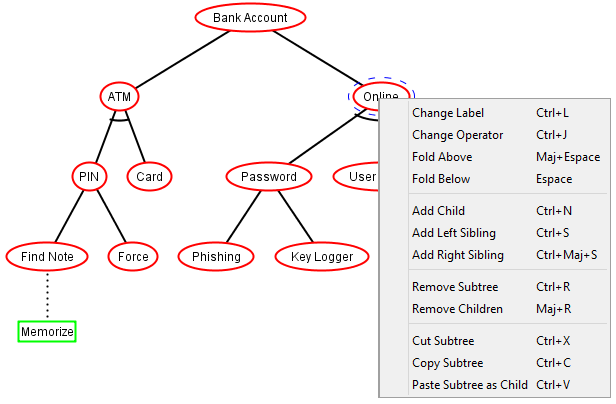
\includegraphics[height=0.7\textwidth]{figure/clicdroit.png}
        \caption{Menu déroulant apparaissant après un clic droit sur un n\oe{}ud.}
        \label{fig:clicdroit}
    \end{figure}

\paragraph{Annulation d'une action} Il s'agit ici d'annuler une ou plusieurs action(s) effectuée(s) précédemment sur l'ADTree courant. Pour cela, il vous suffit tout simplement d'utiliser le raccourci clavier {\sc CTRL+Z} autant de fois que nécessaire, jusqu'à retrouver l'état souhaité pour l'ADTree. Vous pouvez également cliquer sur l'icône \og Undo last action (CTRL+Z) \fg{} en haut à gauche de la fenêtre principale d'ADTool, encadrée en rouge sur la {\sc figure}~\ref{fig:undo}. Les actions pouvant être annulées sont les changements de labels, les ajouts ou suppressions de n\oe{}uds, les changements d'opérateur (conjonction ou disjonction) ainsi que les actions de couper/copier/coller.

\begin{figure}[!h]
        \centering
        
\includegraphics[height=0.17\textwidth]{figure/undo.png}
        \caption{Icône permettant d'annuler l'action précédente.}
        \label{fig:undo}
    \end{figure}

    \newpage
    \bibliographystyle{plain}
    \bibliography{input/biblio}

    % Manoucherie incoming
    \pagevierge
    \ifthenelse{\isodd{\thepage}}
    {\pagevierge}
    {}
    
\includepdf[pages=2]{figure/couv.pdf}
\end{document}
